\section{Integration Strategy}

\subsection{Entry Criteria}
The following conditions have to be verified before entering the integration testing phase in order for it to produce meaningful results.\\

A fundamental initial criterion is that the development of the components and their functionalities proceeds together with the unit testing on such components, so that even when the components are not fully developed, they have already been tested at unit level w.r.t. the fully developed functionalities. 
Given the aforementioned criterion, before entering the integration phase, the development percentage of a component must be at least 90\% and the main functionalities required to test its integration w.r.t. another component of the system must be fully developed.\\

The integration process can start when these conditions are met by the system development
\begin{itemize}
	\item 100\% of development on the \emph{Data Provider} component
	\item 90\% of development on the \emph{Event Broker} and \emph{Car Handler} components
	\item 80\% of development on the \emph{Rent Manager} component
	\item 60\% of development on the \emph{Maintenance Manager} component
	\item 40\% of development on the \emph{User Information Manager} and \emph{Access Manager} components
	\item 30\% of development on the \emph{User Application Server}, \emph{User Application}, \emph{Customer Care Server} and \emph{Customer Care Application} components
\end{itemize}

\subsection{Elements to be integrated}
In this section we identify the components and subcomponents to be integrated and add some details about their specific integration.\\

As specified in the design document, some component of the PowerEnJoy system such as the \emph{Rent Manager} and the \emph{Maintenance Manager} are rather complex and thus its internal subcomponents need to be integrated before proceeding with the integration of entire components with other components of the system.\\

The following components will be integrated to obtain the subsystem related to the Maintenance functionalities:

\begin{itemize}
	\item \emph{Maintenance Manager}
	\item \emph{Event Broker}
	\item \emph{Data Provider}
	\item \emph{Car Handler}
\end{itemize}

The following components will be integrated to obtain the subsystem related to the User Application functionalities:

\begin{itemize}
	\item \emph{User Application}
	\item \emph{UserApp Server}
	\item \emph{Access Manager}
	\item \emph{Rent Manager}
	\item \emph{User Information Manager}
	\item \emph{Data Provider}
	\item \emph{Car Handler}
	\item \emph{Event Broker}
\end{itemize}

The following components will be integrated to obtain the subsystem related to the Customer Care functionalities:

\begin{itemize}
	\item \emph{Customer Care Application}
	\item \emph{Customer Care Server}
	\item \emph{User Information Manager}
	\item \emph{Data Provider}
\end{itemize}

\paragraph{Notes}
The external components like the \emph{DBMS} and the external APIs are products that are not developed by us and that we suppose already completely tested; however we decided to include them in the integration testing by firstly testing the external component's interfaces on their own, and the by proceeding to test them when integrated with PowerEnJoy components.\\
In the same way the Maintenance Manger will be tested as a component integrated with our system and then it will be tested through the Maintenance API it provides to the maintenance company. 

\subsection{Integration Testing Strategy} \label{sec:intStrategy}
A Bottom-up approach was chosen because most of the functionalities and the complexity is located in lower level components of our system, hence it is a better choice to test them first and ensure that they work well together before higher level components.

\clearpage
\subsection{Sequence of Component Integration}
This section describes the proposed plan for the integration test phase of the PowerEnJoy system.

\subsubsection{Overall Component Integration Diagram}  \label{sec:overallPrecedences}
The diagram above shows the needed precedences in the integration phase between the main components of the system taking into account the integration testing strategy chosen.

\paragraph{NOTES} In the following diagram we represent with arrows the precedences needed between the components, the purpose is to indicate that following the strategy chosen a component can be integrated with another one only if that component has already been integrated with all the component it needs to be integrated with (arrows point from the \emph{<need integration>} component to the \emph{<needed integration>} one, numbers are shown to clearify order of the integration and steps that are possibly made in parallel).

	\begin{figure}[h]
			\centering
			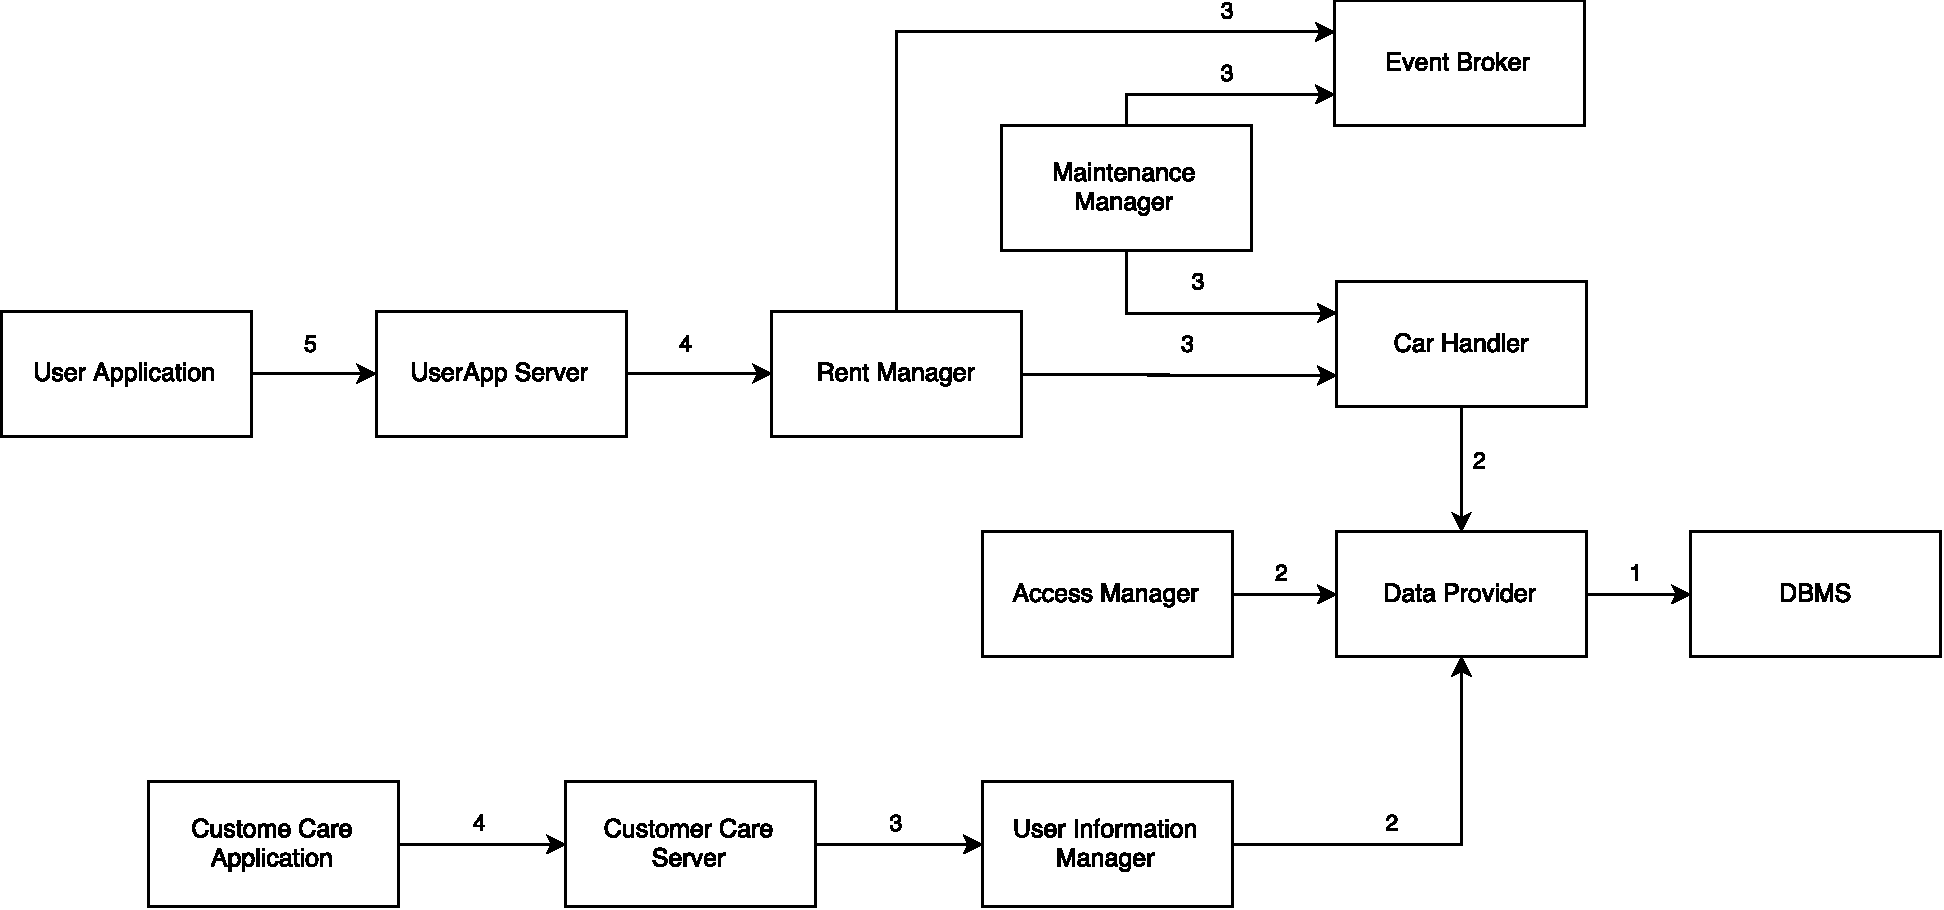
\includegraphics[width=\linewidth]{img/overallIntegration}
			\caption{
				\label{fig:overallIntegration} 
				\emph{Overall Component Integration Diagram}
			}
	\end{figure}
	
\clearpage
\subsubsection{Subcomponent Integration}
In the \emph{PowerEnJoy: Design Document}\cite{DD} some high-level components are described deeply through the definition of the subcomponents composing them.
In this section are shown the diagram of the precedences between the subcomponents to integrate them. We assume that when the high-level component enters the integration sequence presented they have been fully tested inside considering them as a single component unit-level tested to be integrated.

\paragraph{RentManager} 
The diagram above shows the needed precedences in the integration phase between the \emph{RentManager} subcomponents.
\paragraph{}

		\begin{figure}[h]
			\centering
			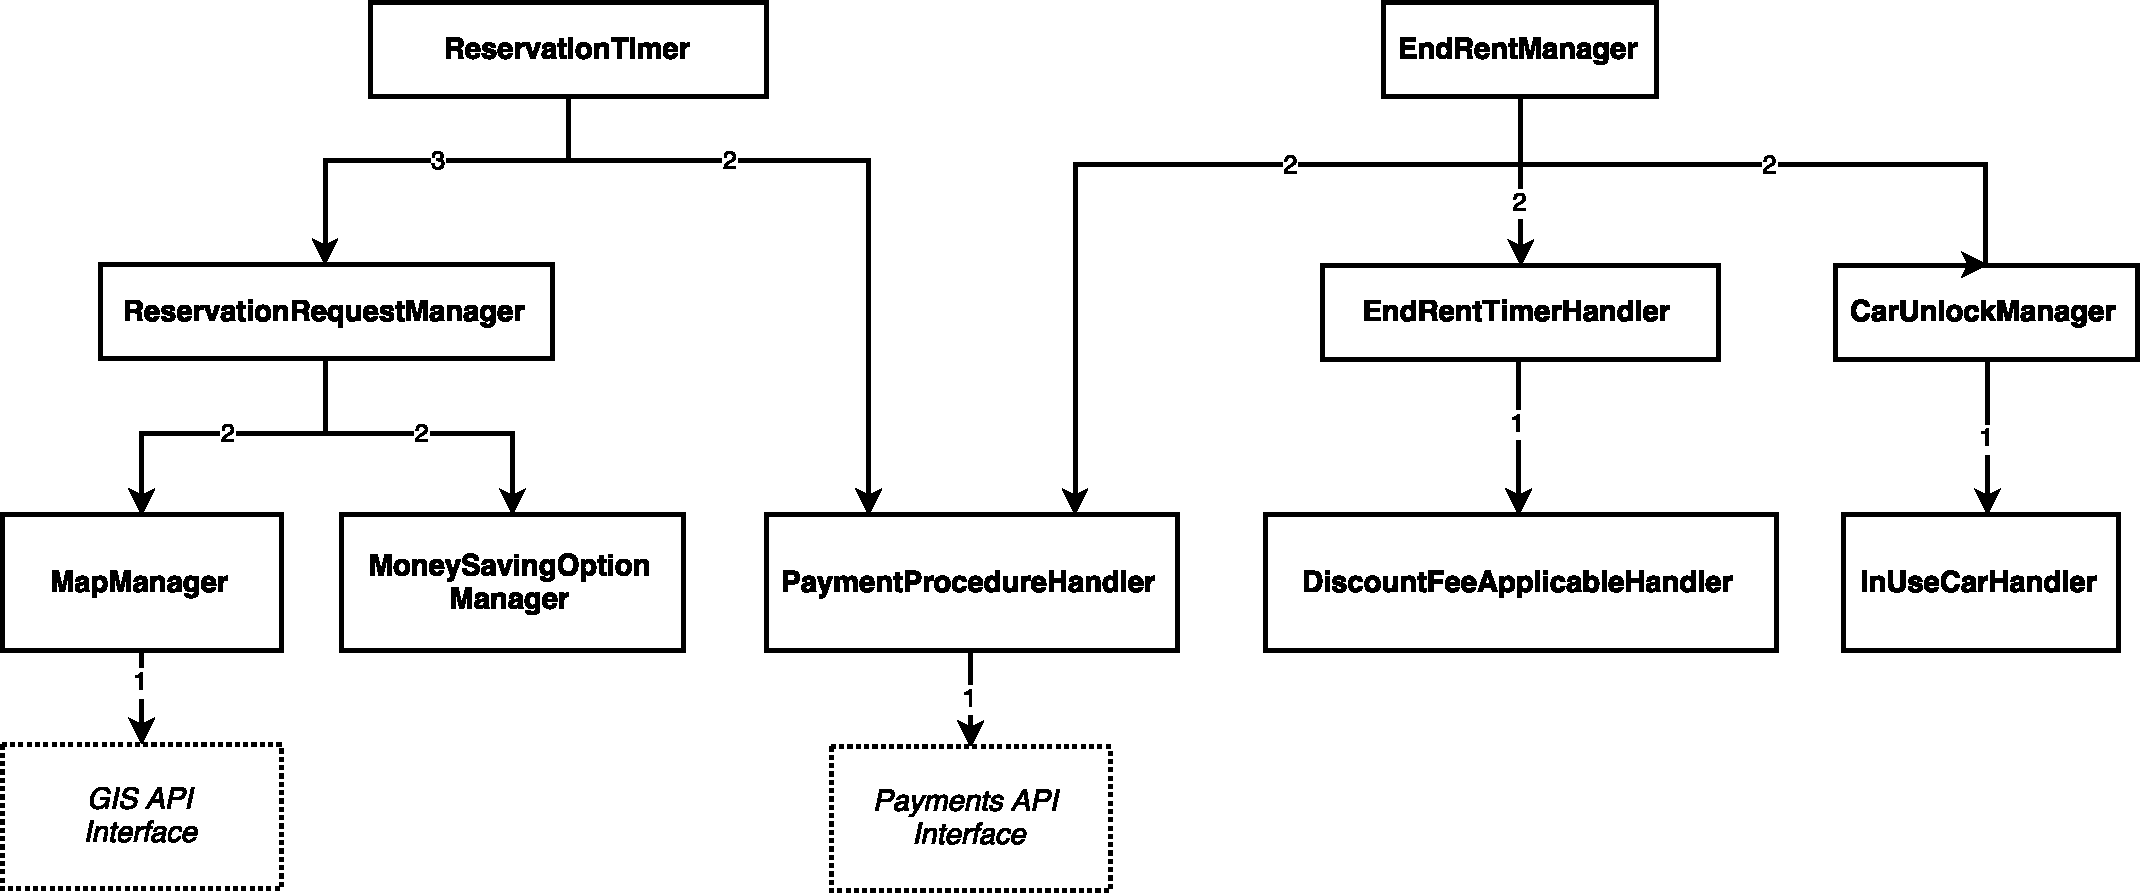
\includegraphics[width=\linewidth]{img/rentManagerIntegration}
			\caption{
				\label{fig:rentManagerIntegration} 
				\emph{RentManager subcomponents integration}
			}
		\end{figure}
		
\paragraph{MaintenanceManager} 
The diagram above shows the needed precedences in the integration phase between the \emph{MaintenanceManager} subcomponents.
\paragraph{}

		\begin{figure}[h]
			\centering
			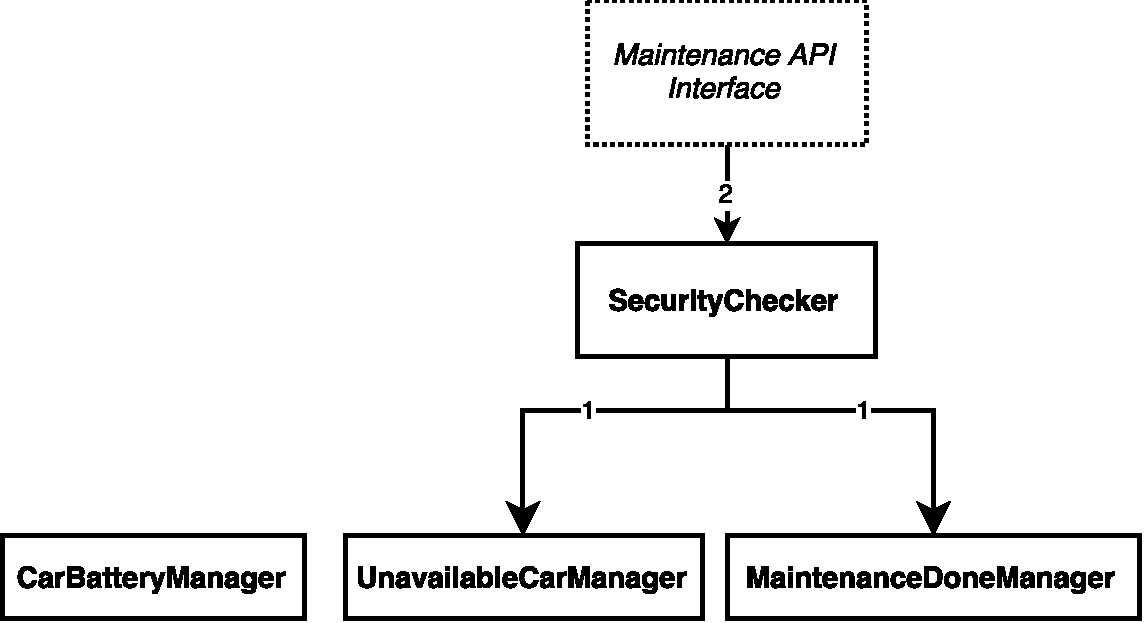
\includegraphics[width=0.6\linewidth]{img/maintenanceIntegration}
			\caption{
				\label{fig:maintenanceIntegration} 
				\emph{MaintenanceManager subcomponents integration}
			}
		\end{figure}
		
\paragraph{UserInformationManager} 
The diagram above shows the needed precedences in the integration phase inside the \emph{UserInformationManager} subcomponents.
\paragraph{}

		\begin{figure}[h]
			\centering
			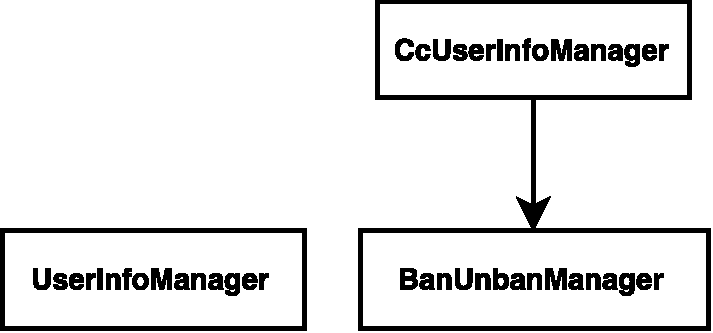
\includegraphics[width=0.4\linewidth]{img/userIntegration}
			\caption{
				\label{fig:userIntegration} 
				\emph{UserInformationManager subcomponents integration}
			}
		\end{figure}

\subsubsection{Component Integration}
This section describes the sequence proposed to plan the integration test of all the components of the PowerEnJoy system. As specified in the \hyperref[sec:intStrategy]{Integration Testing Strategy section} we decide to start the bottom-up integration from the components related to the critical functionality of the system (such as the communication with cars); even if the steps are proposed sequentially following these criteria, it is clear the sequence proposed presents the possibility to make same integration steps in parallel given the needed precedences between components presented in the \hyperref[sec:overallPrecedences]{Overall Component Integration Diagram}.

\paragraph{DataProvider} 
...
\paragraph{}

		\begin{figure}[h]
			\centering
			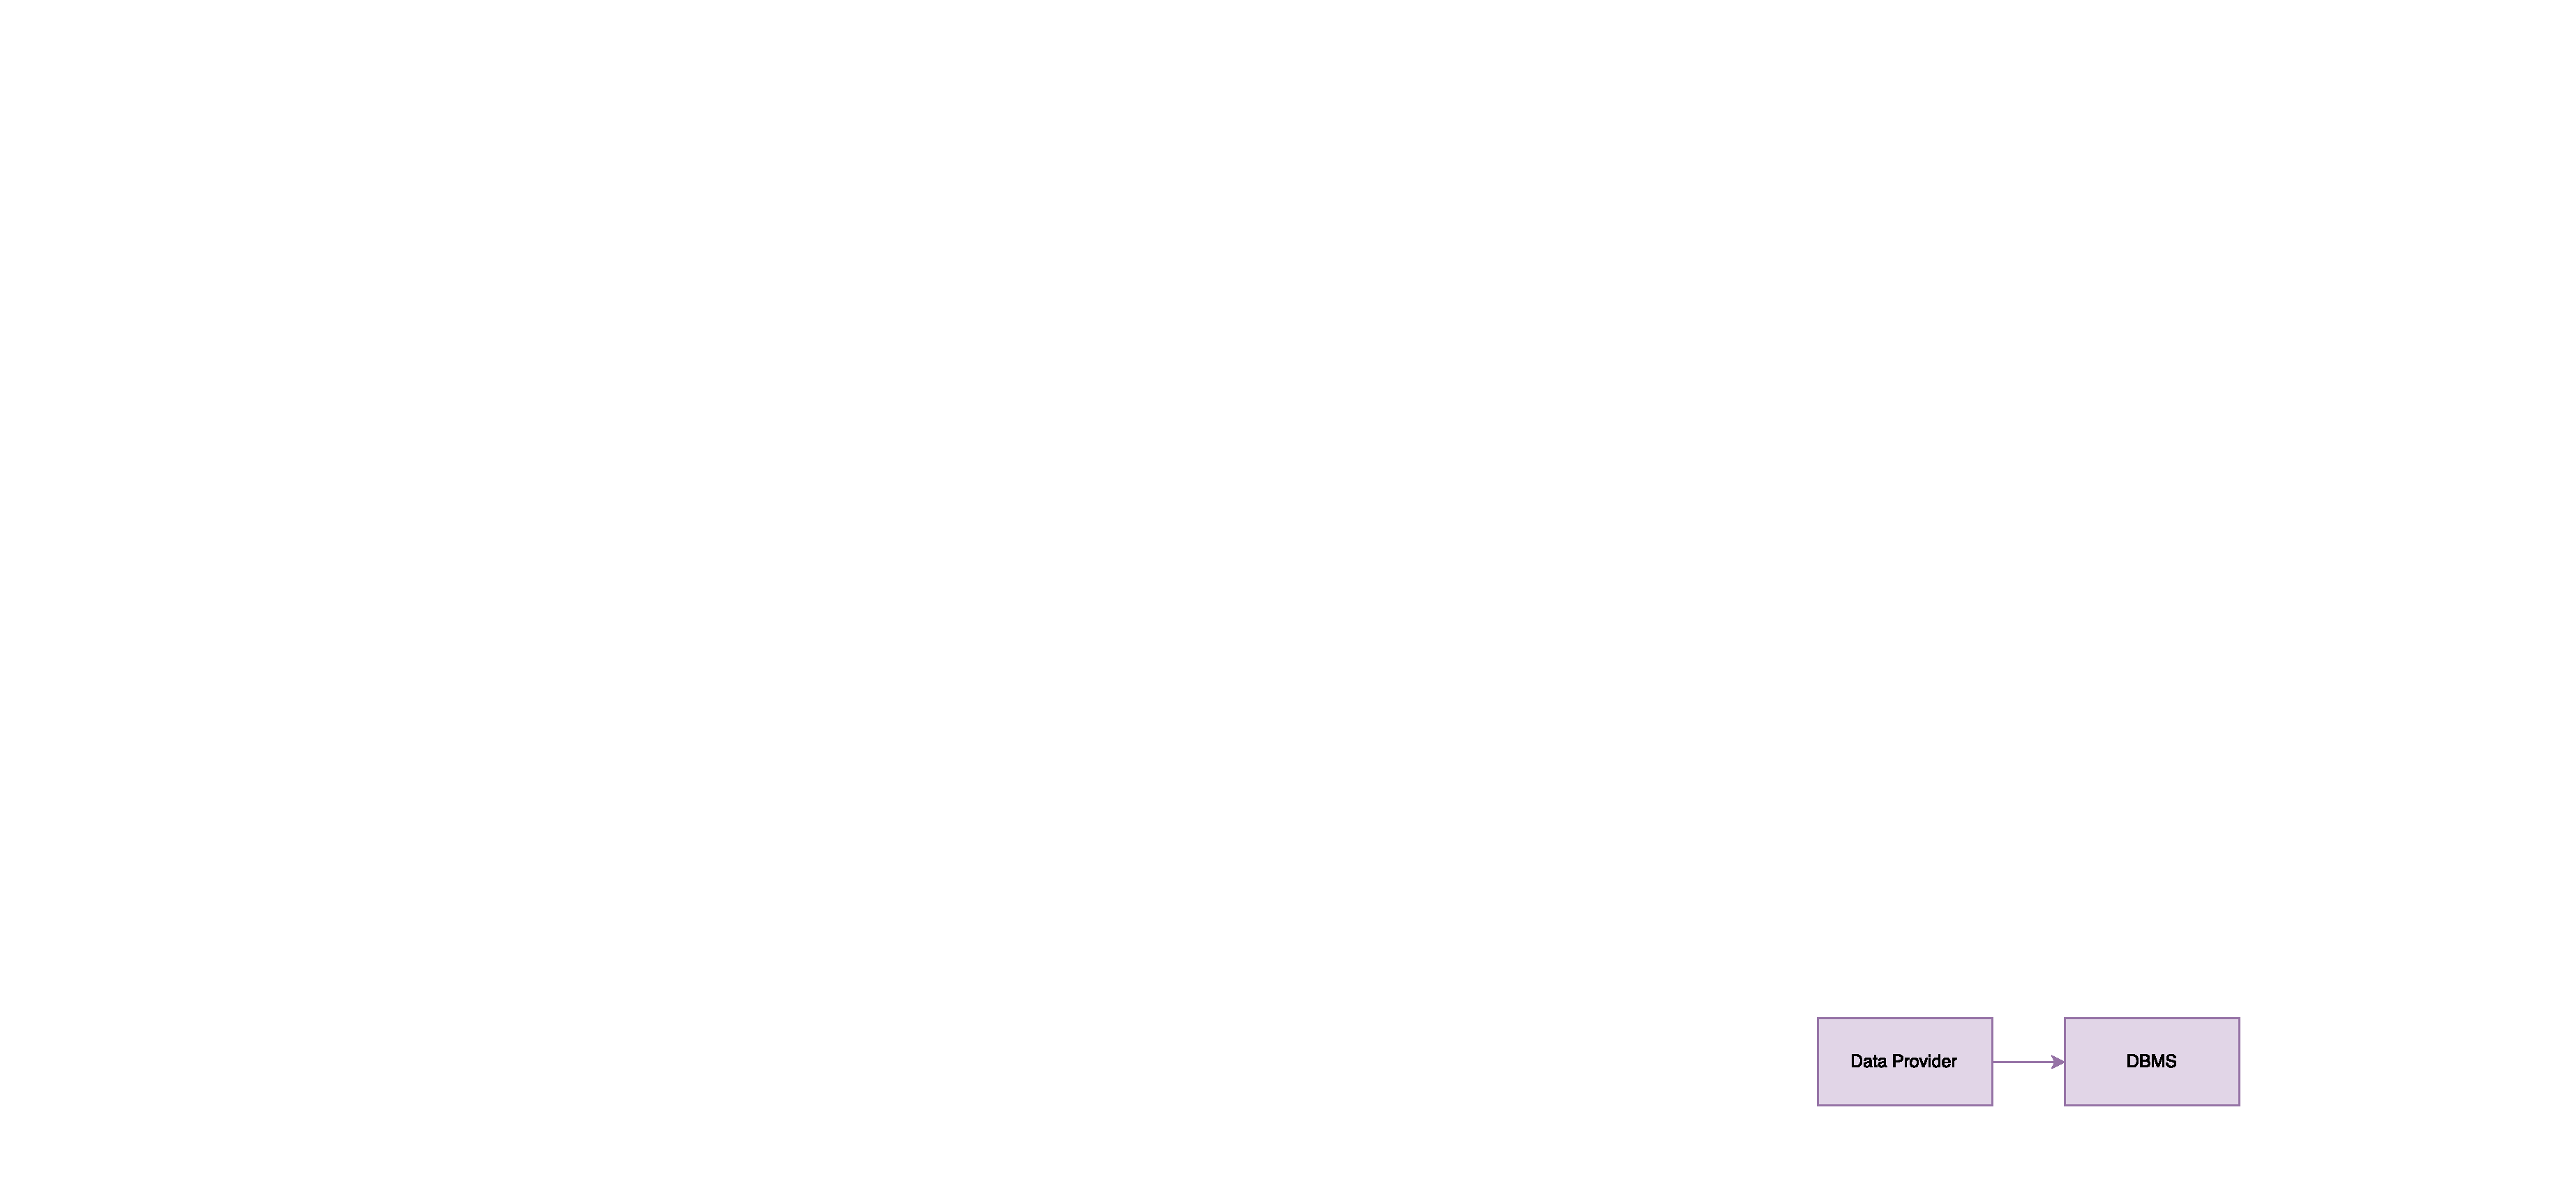
\includegraphics[width=0.6\linewidth]{img/Integration1}
			\caption{
				\label{fig:dataProvider} 
				\emph{DataProvider integration}
			}
		\end{figure}

\paragraph{EventBroker and CarHandler} 
...
\paragraph{}
		
		\begin{figure}[h]
			\centering
			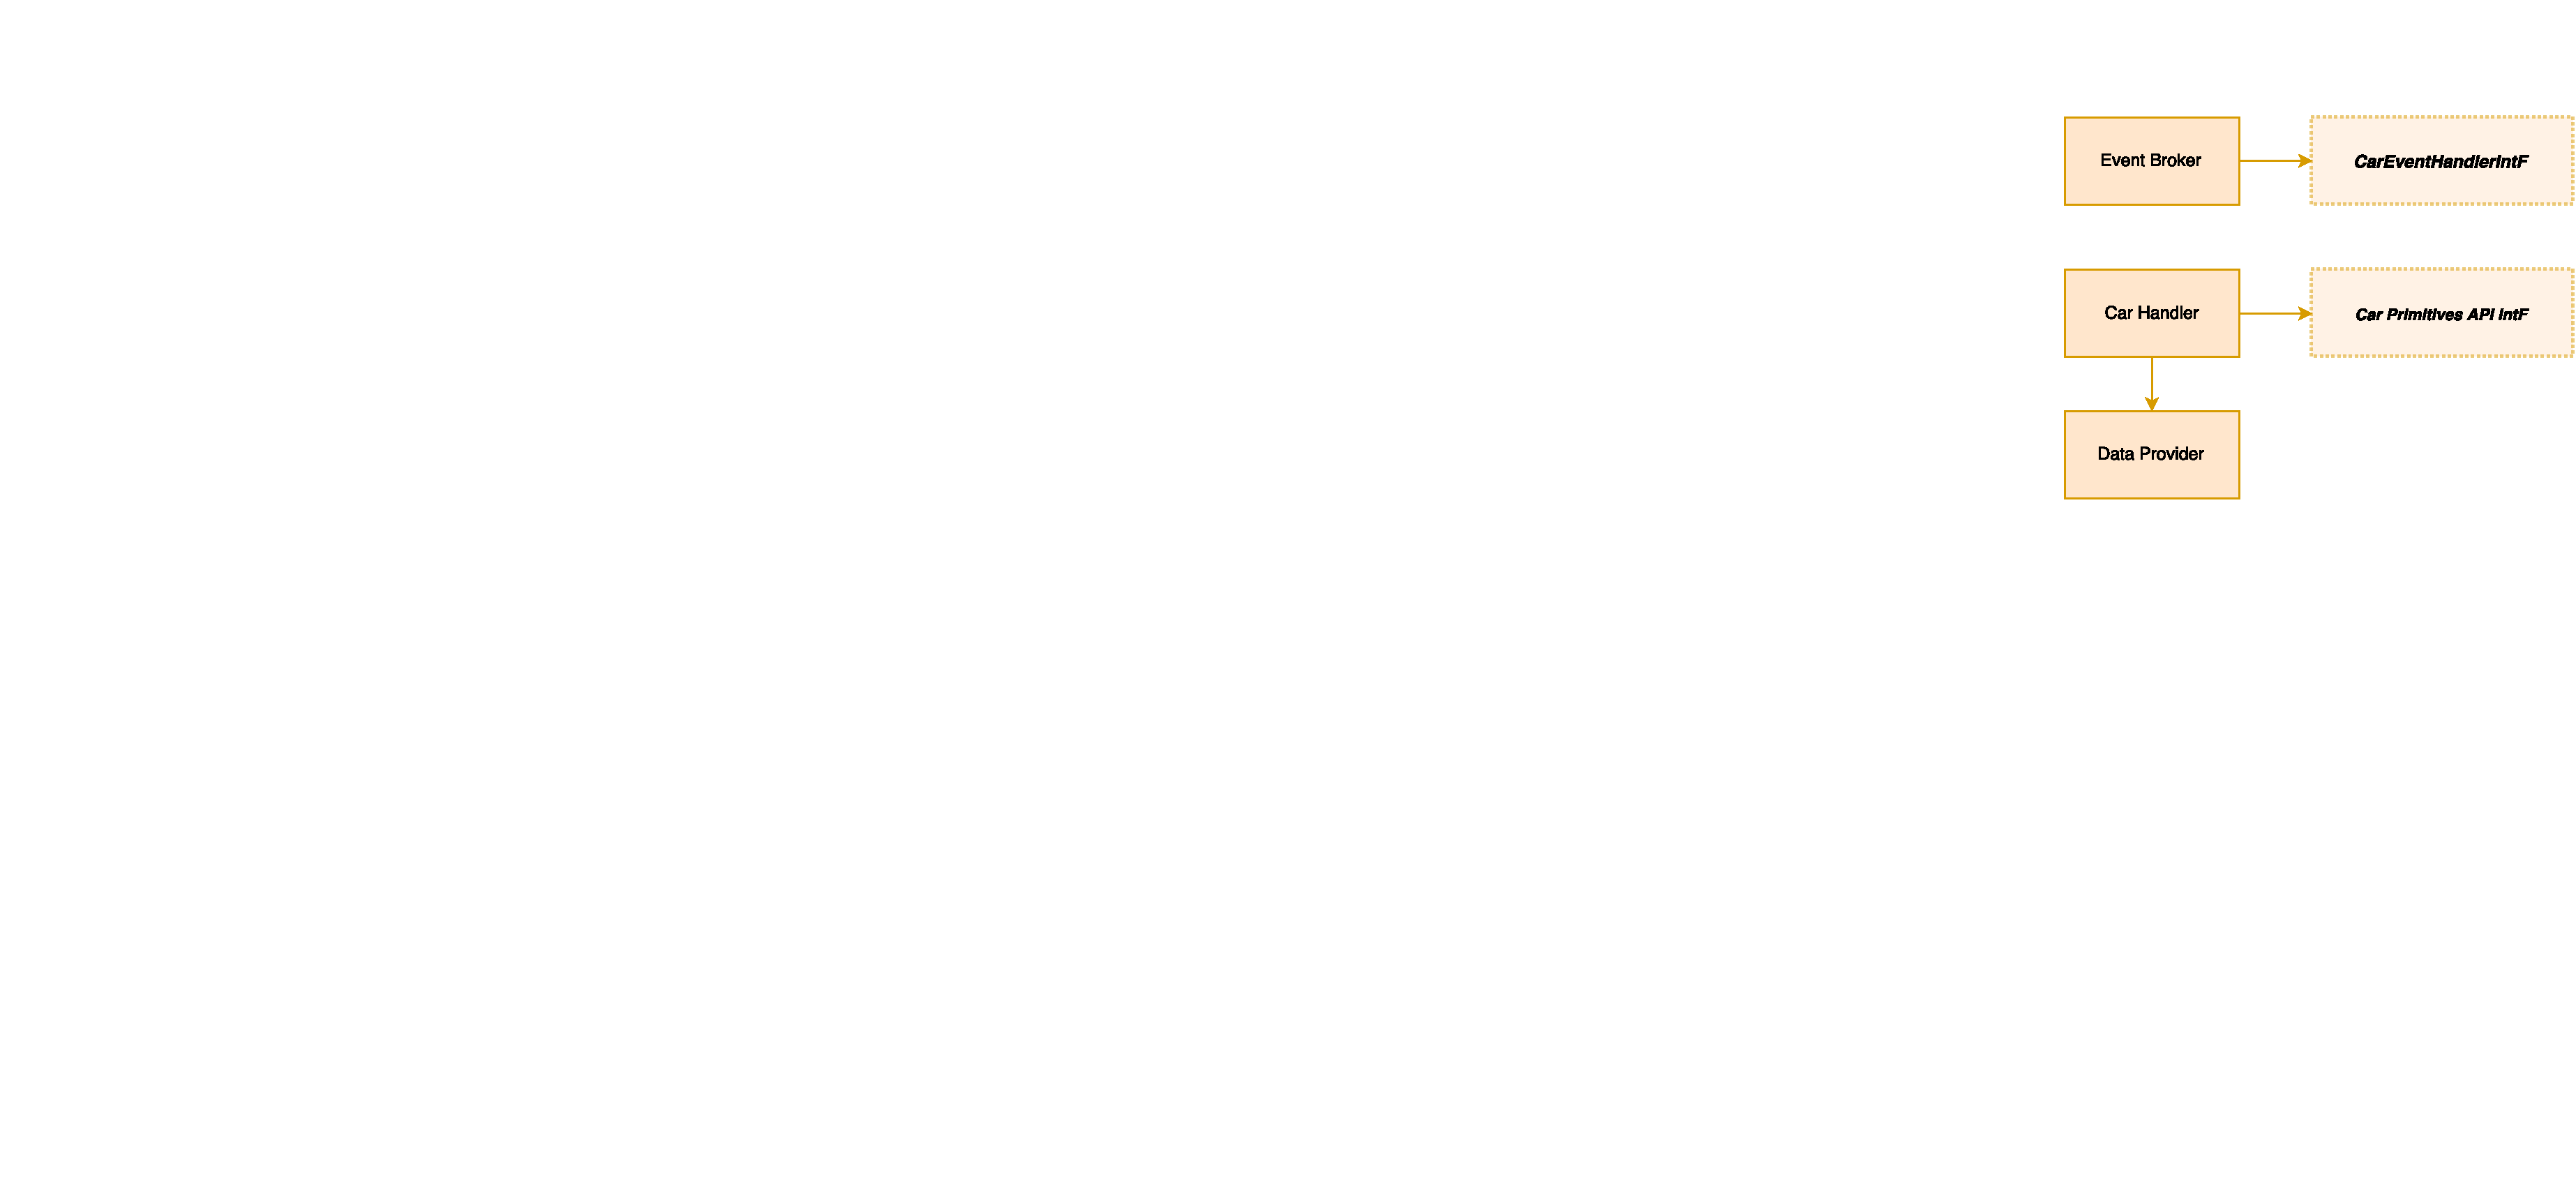
\includegraphics[width=0.6\linewidth]{img/Integration2a}
			\caption{
				\label{fig:eventBrokerCarHandler} 
				\emph{EventBroker and CarHandler integration}
			}
		\end{figure}

\paragraph{UserInformationManager and AccessManager} 
...
\paragraph{}
		
		\begin{figure}[h]
			\centering
			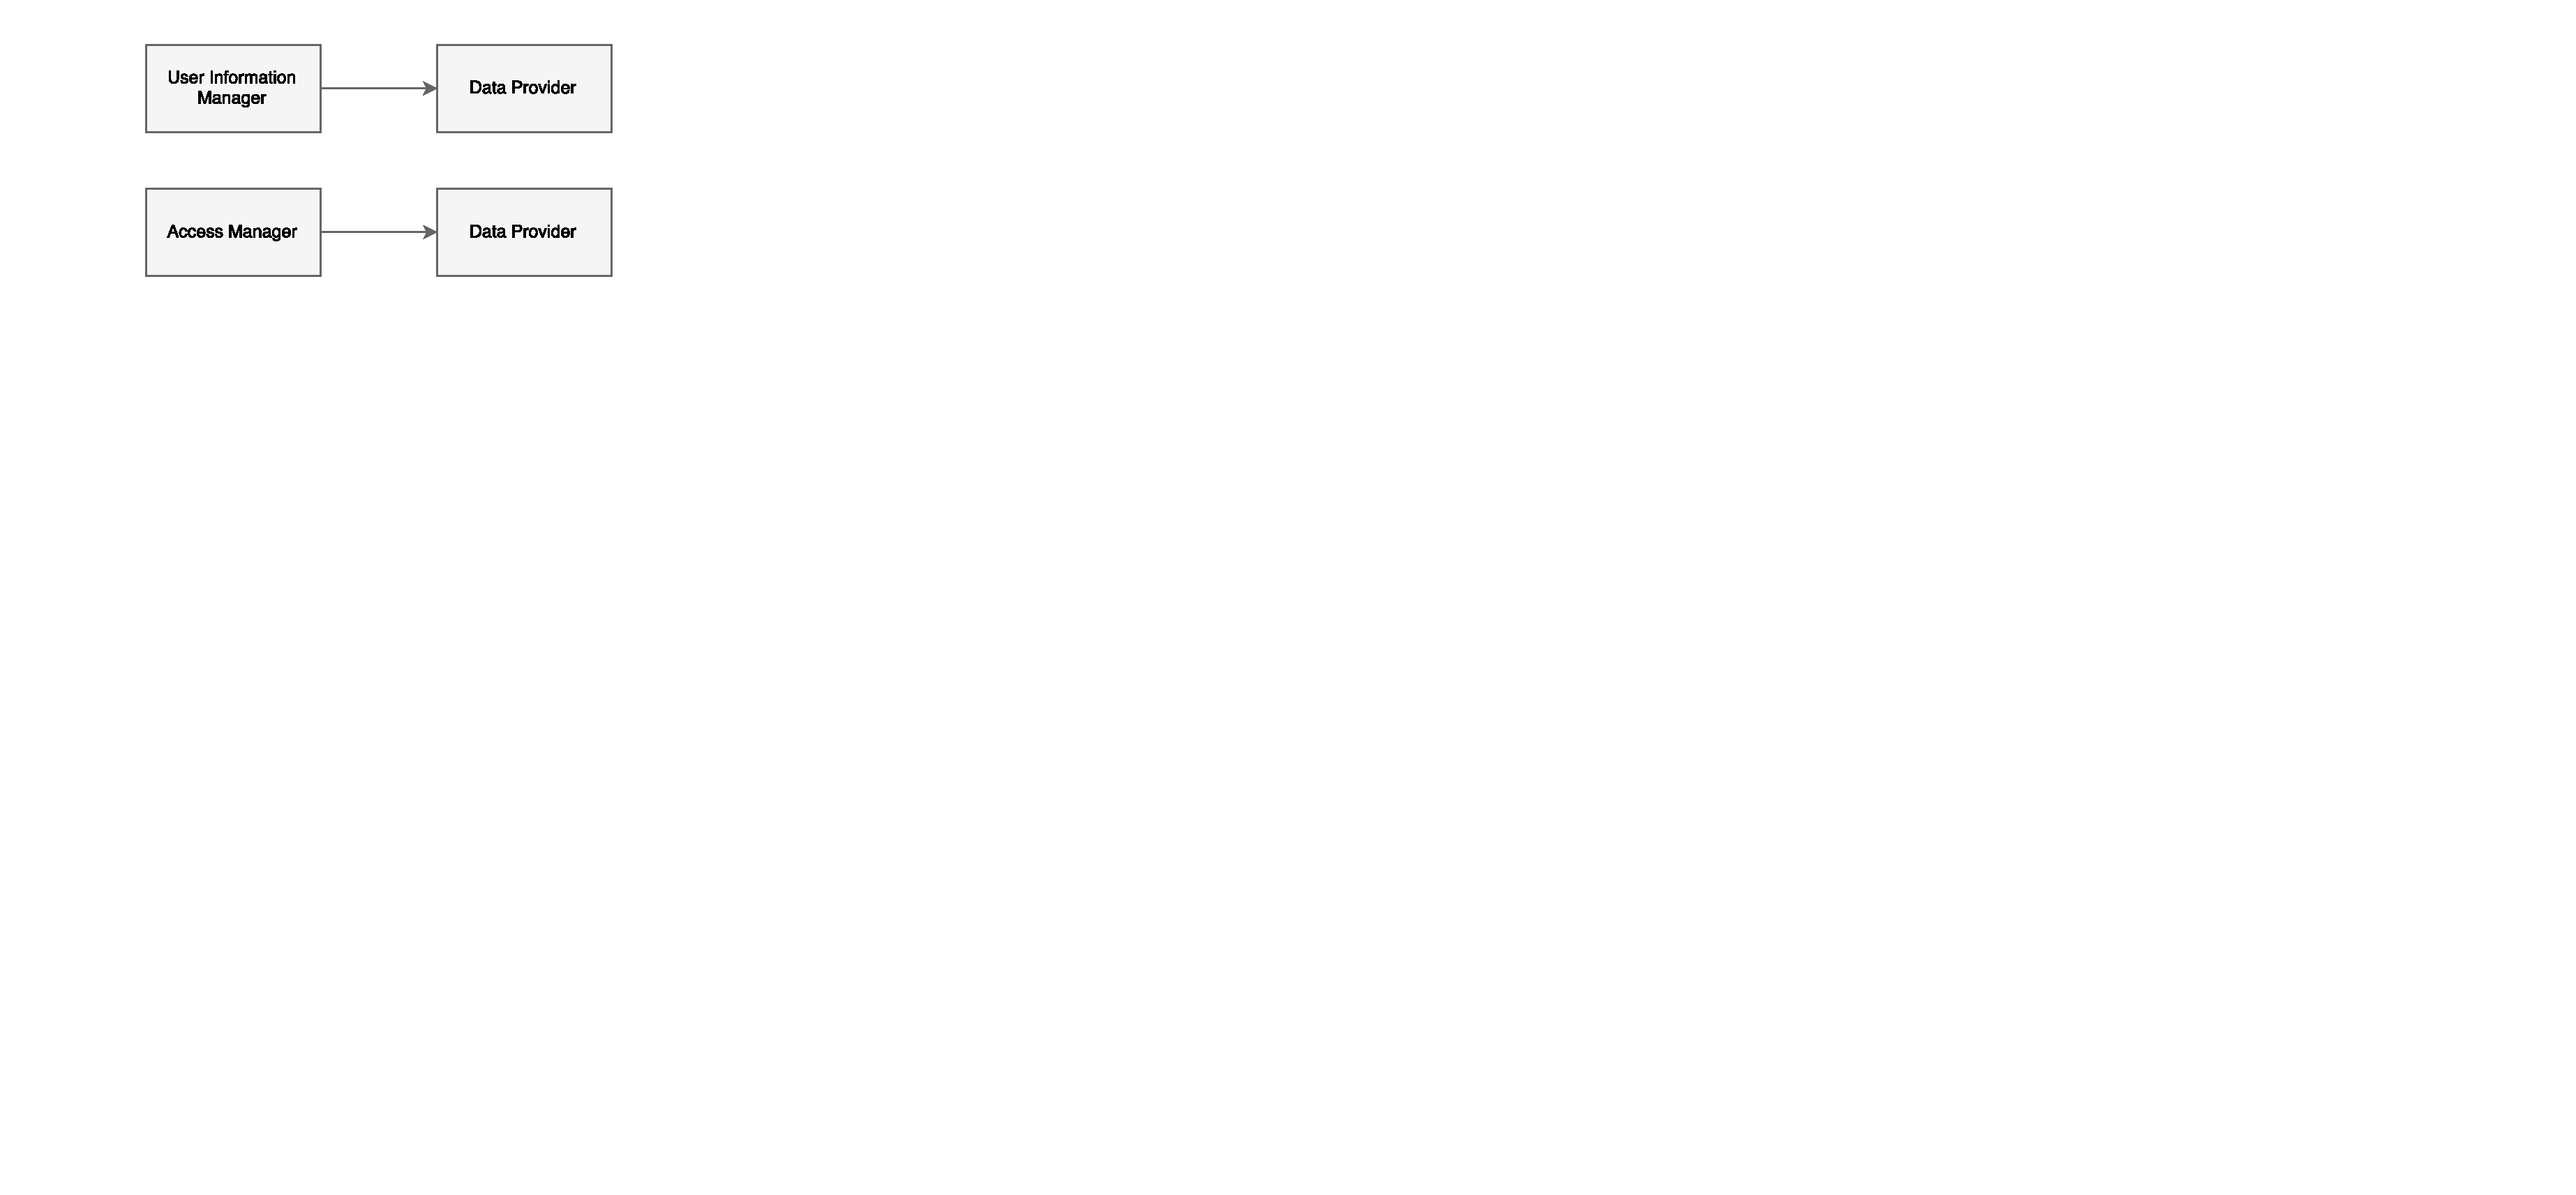
\includegraphics[width=0.6\linewidth]{img/Integration2b}
			\caption{
				\label{fig:userInfoAccessManager} 
				\emph{UserInformationManager and AccessManager integration}
			}
		\end{figure}
		
\paragraph{RentManager} 
...
\paragraph{}
		
		\begin{figure}[h]
			\centering
			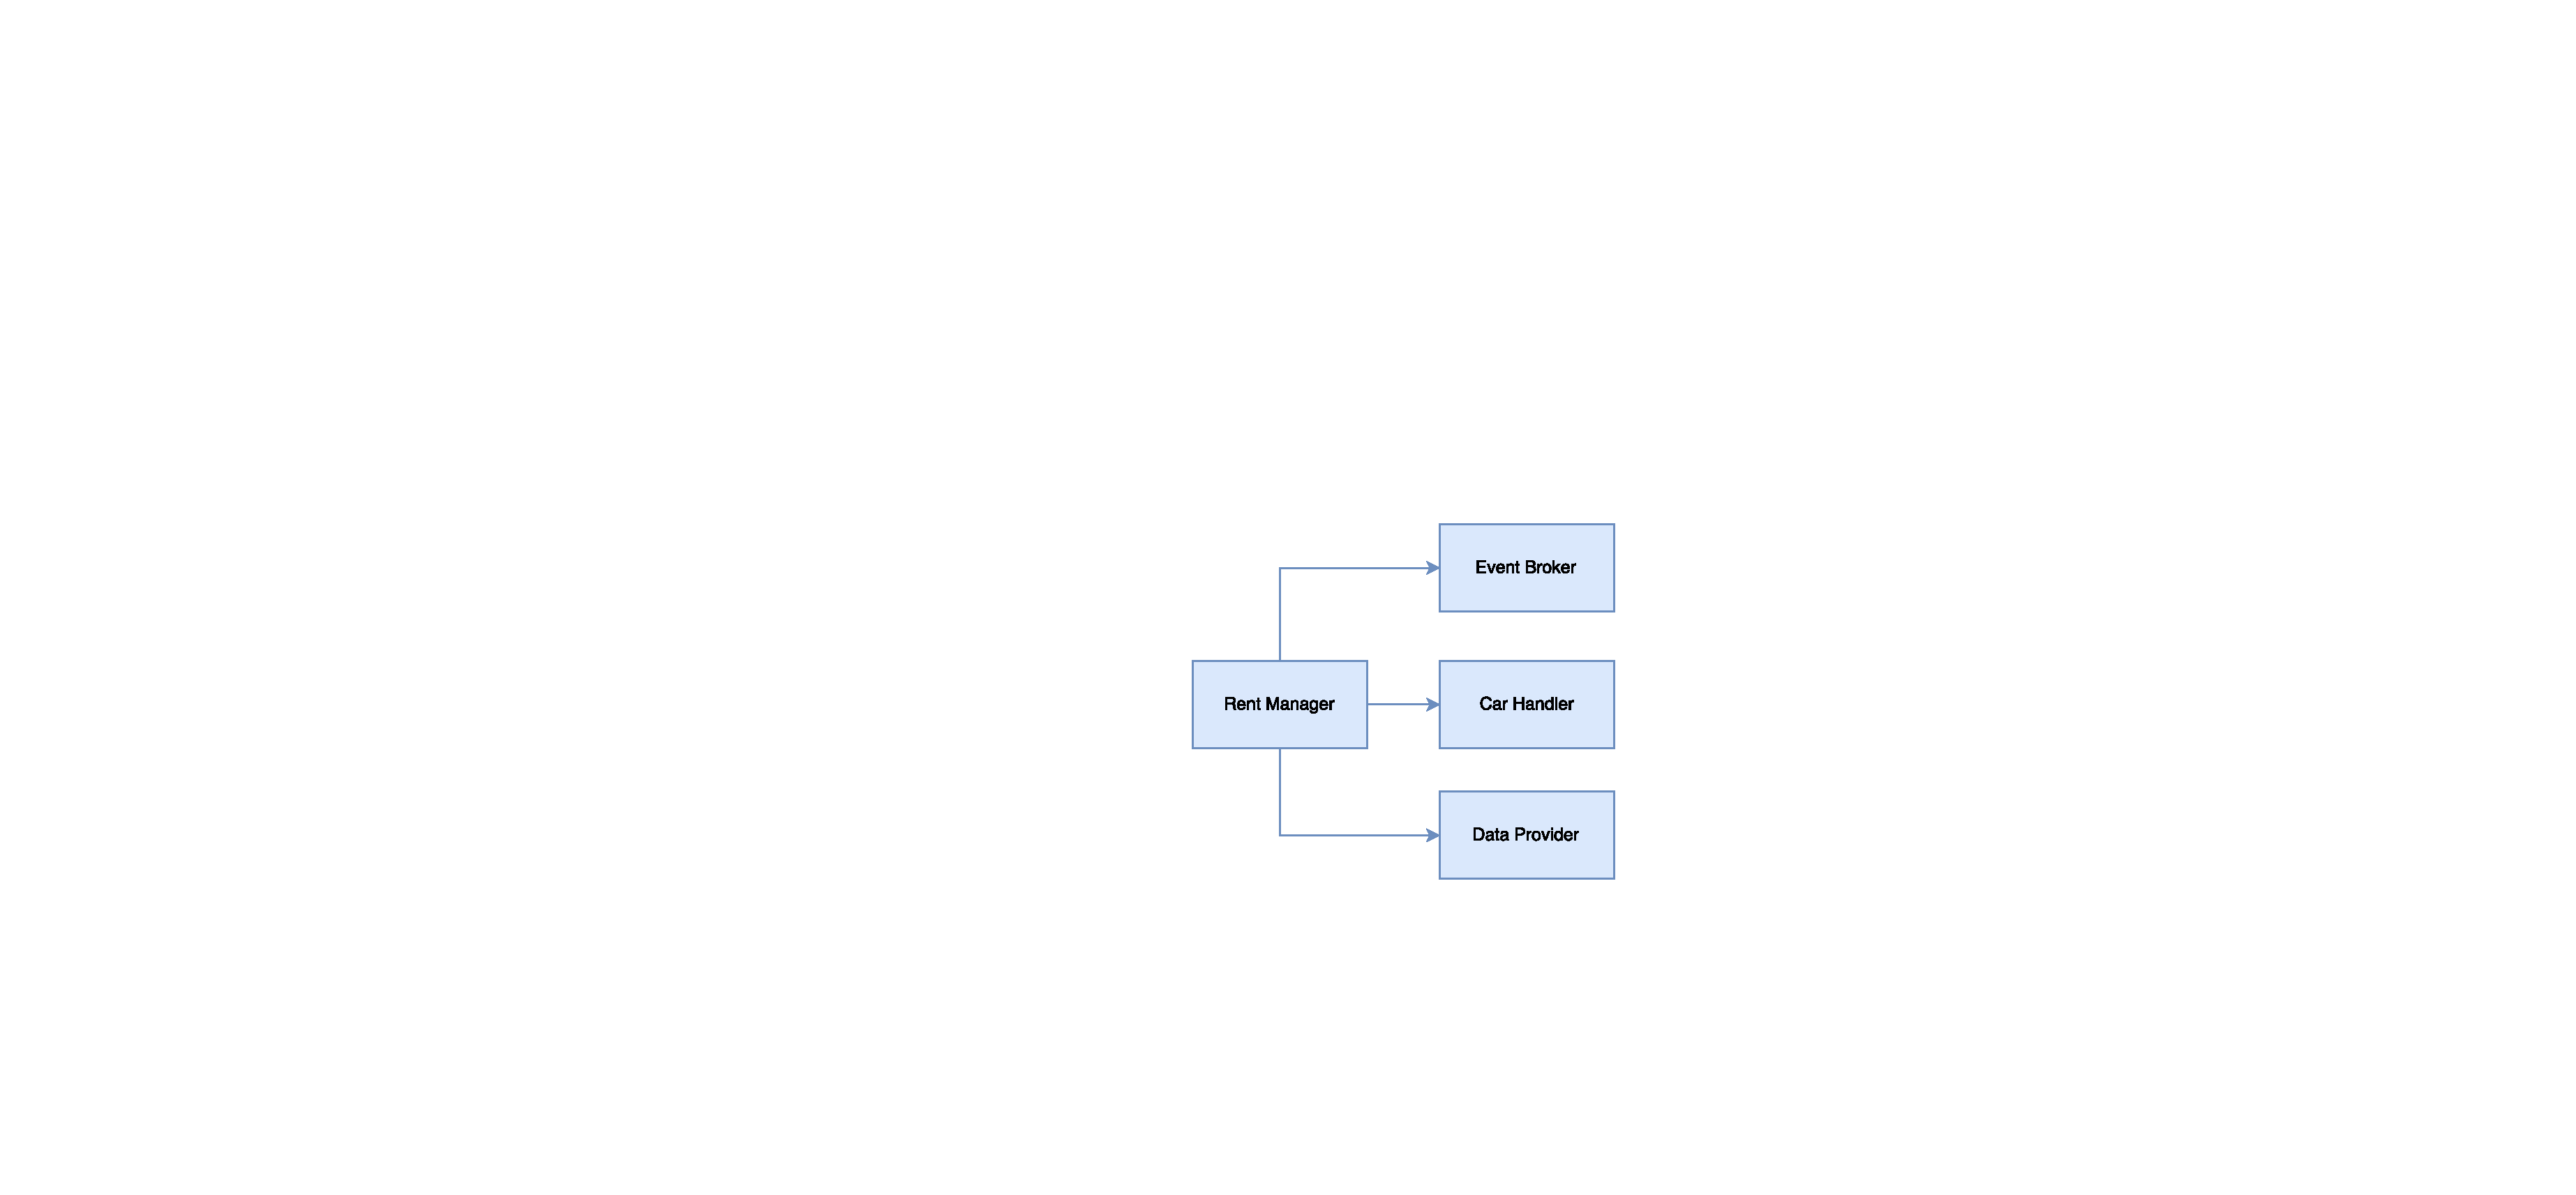
\includegraphics[width=0.8\linewidth]{img/Integration3a}
			\caption{
				\label{fig:rentManager} 
				\emph{RentManager integration}
			}
		\end{figure}

\paragraph{MaintenanceManager} 
...
\paragraph{}
		
		\begin{figure}[h]
			\centering
			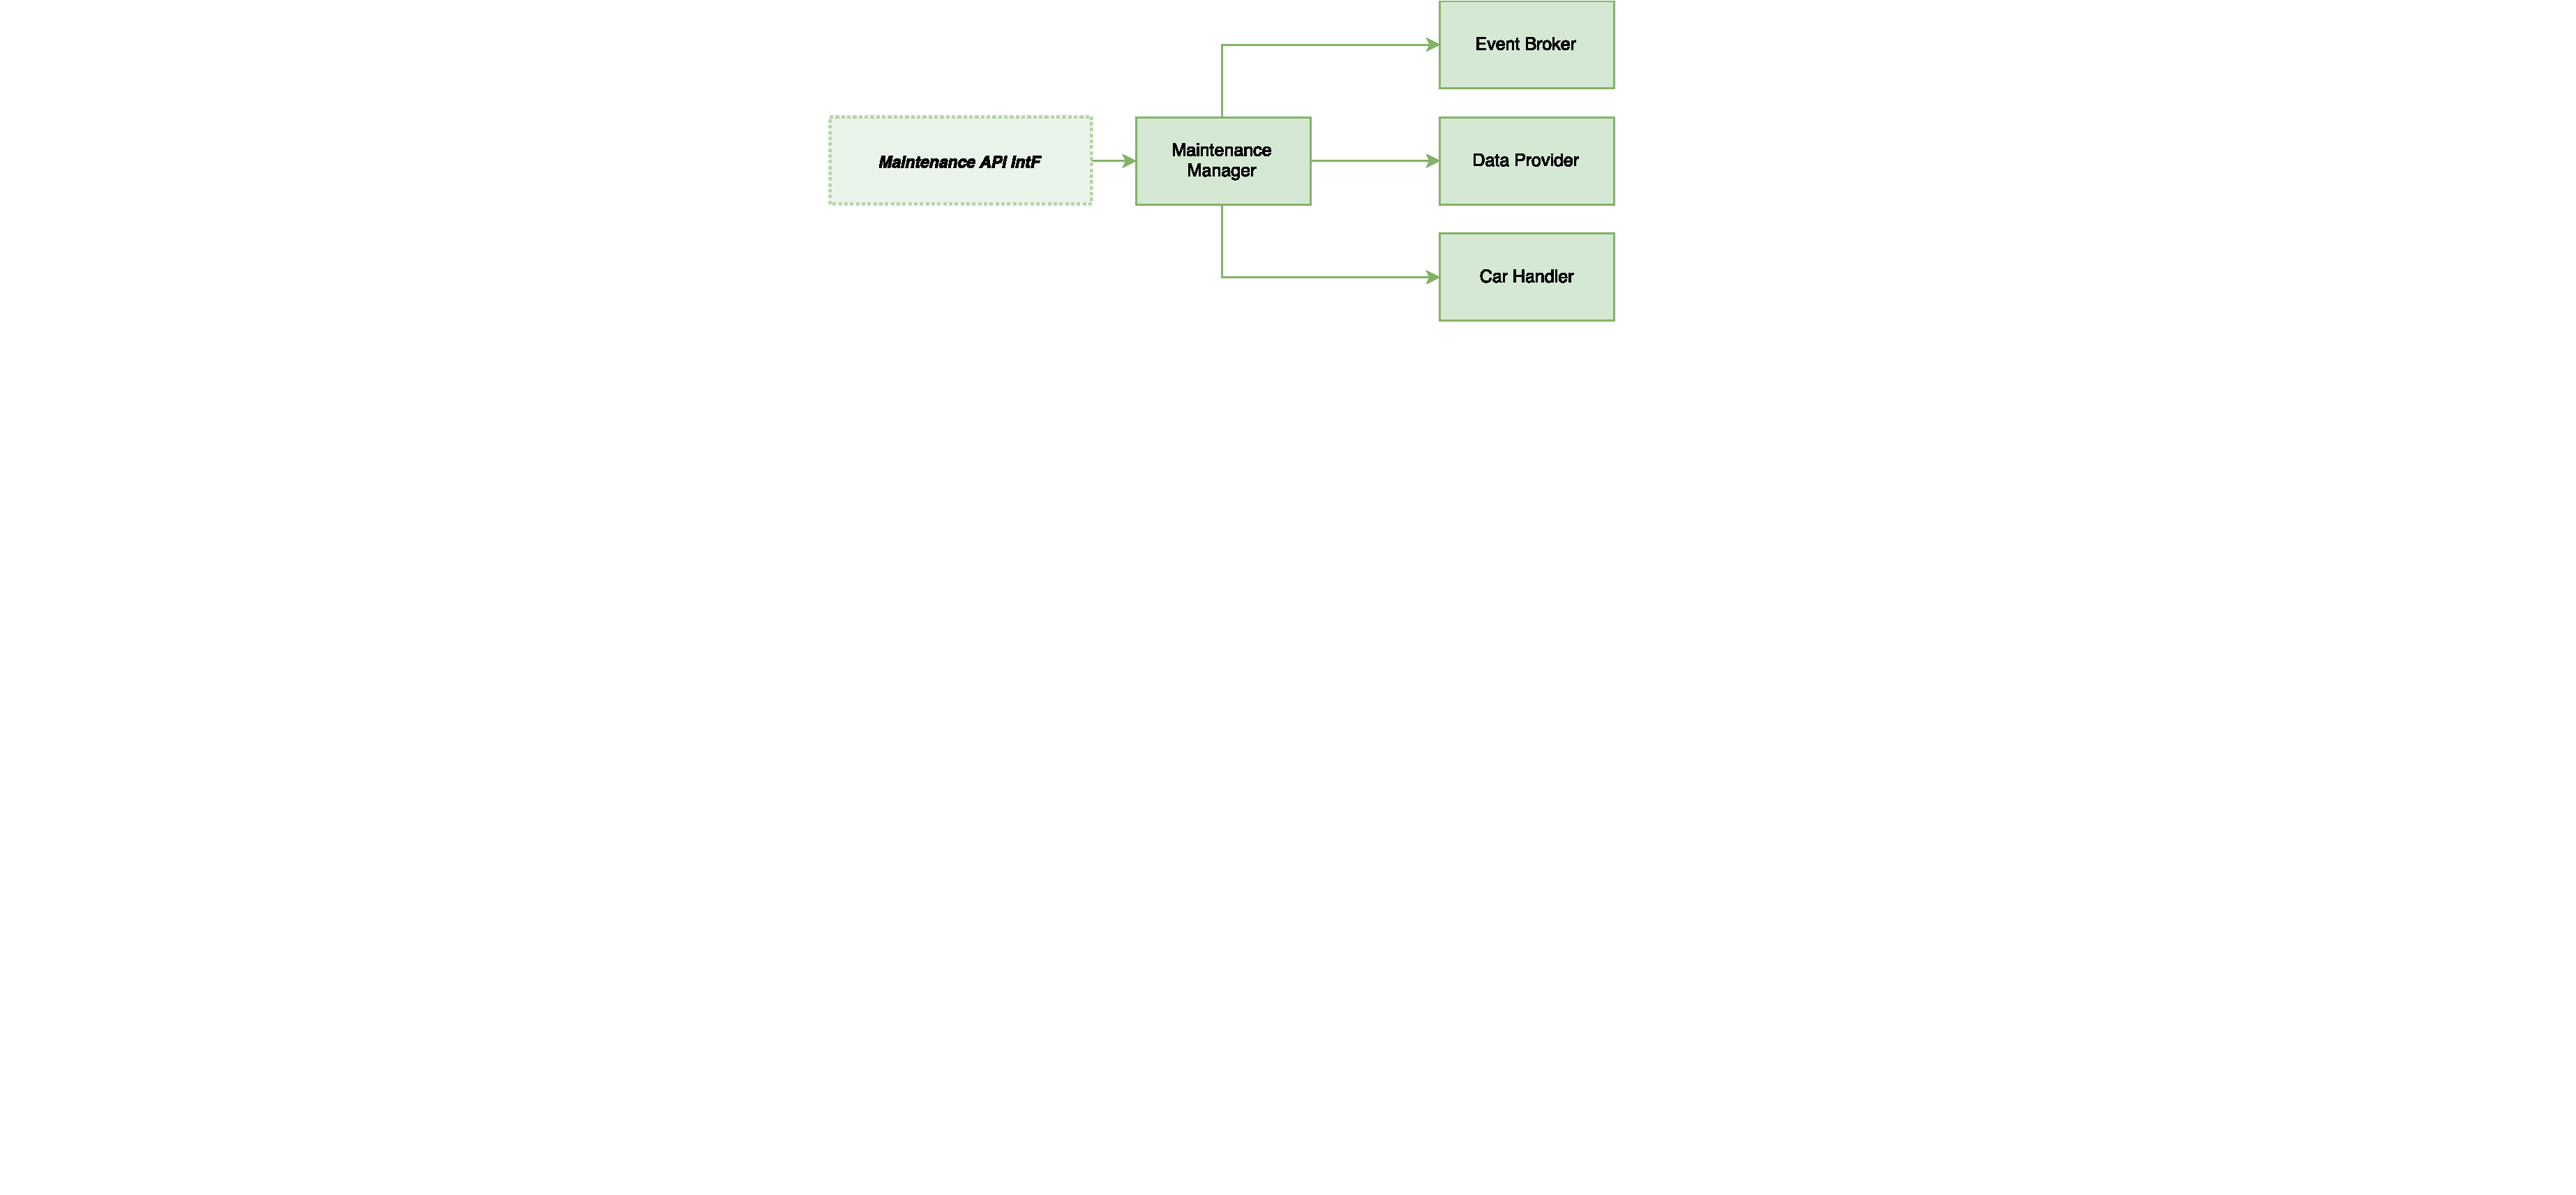
\includegraphics[width=0.8\linewidth]{img/Integration3b}
			\caption{
				\label{fig:maintenanceManager} 
				\emph{MaintenanceManager integration}
			}
		\end{figure}
		
\paragraph{CustomerCare Application and Server} 
...
\paragraph{}
		
		\begin{figure}[h]
			\centering
			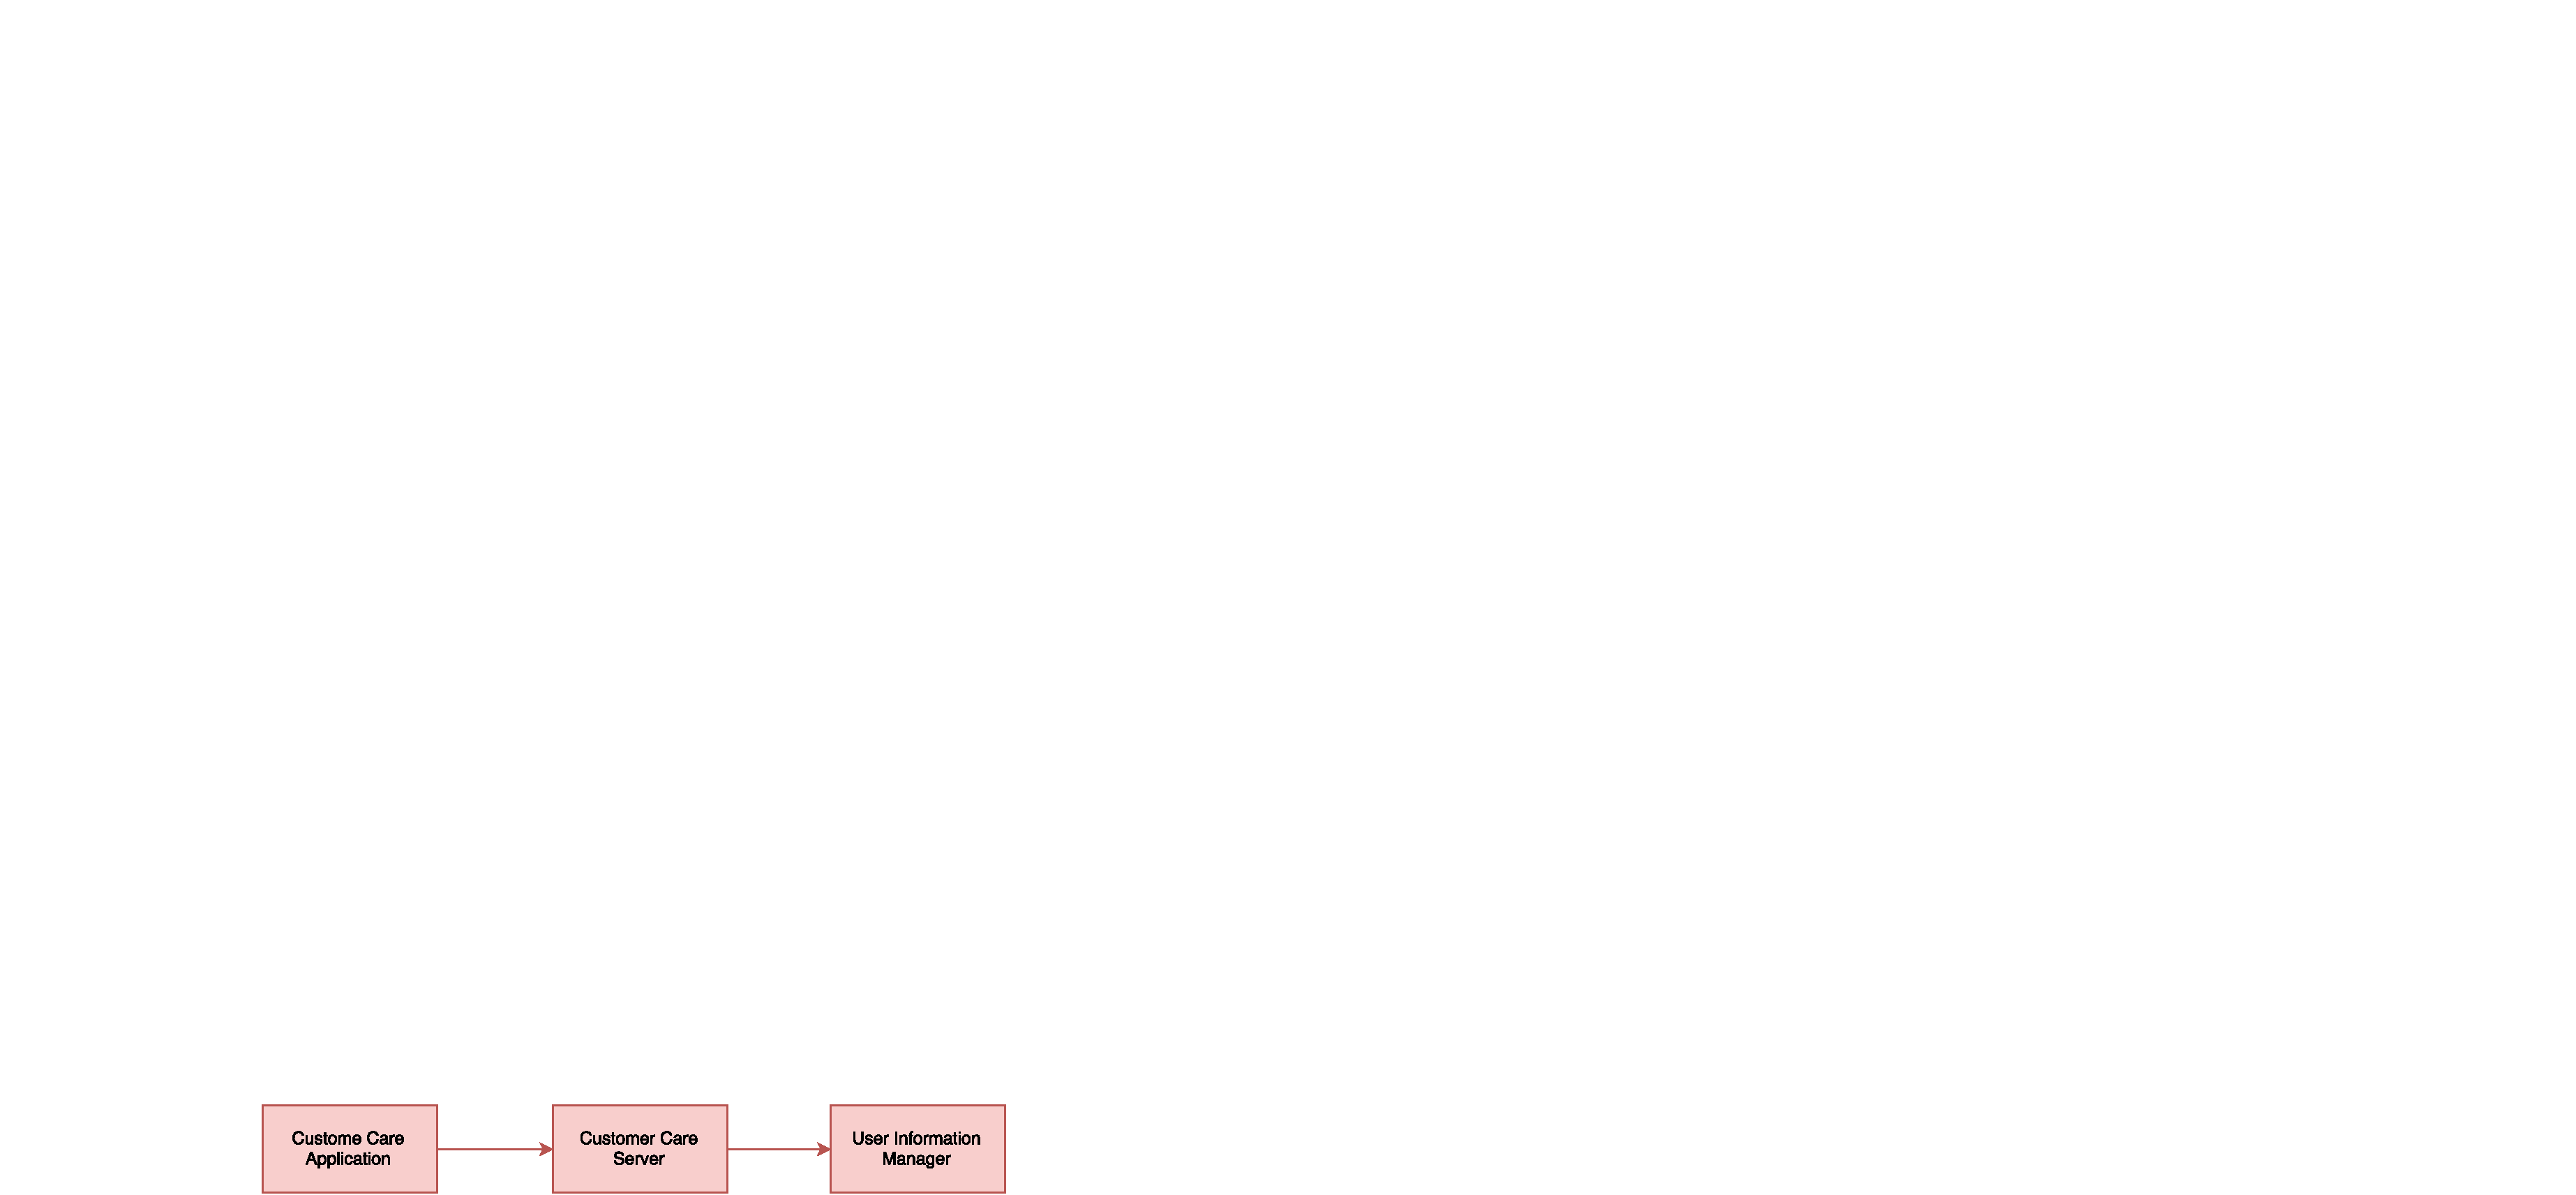
\includegraphics[width=0.8\linewidth]{img/Integration3c}
			\caption{
				\label{fig:ccAppServer} 
				\emph{CustomerCare Application and Server integration}
			}
		\end{figure}
		
\paragraph{User Application and Server} 
...
\paragraph{}
		
		\begin{figure}[h]
			\centering
			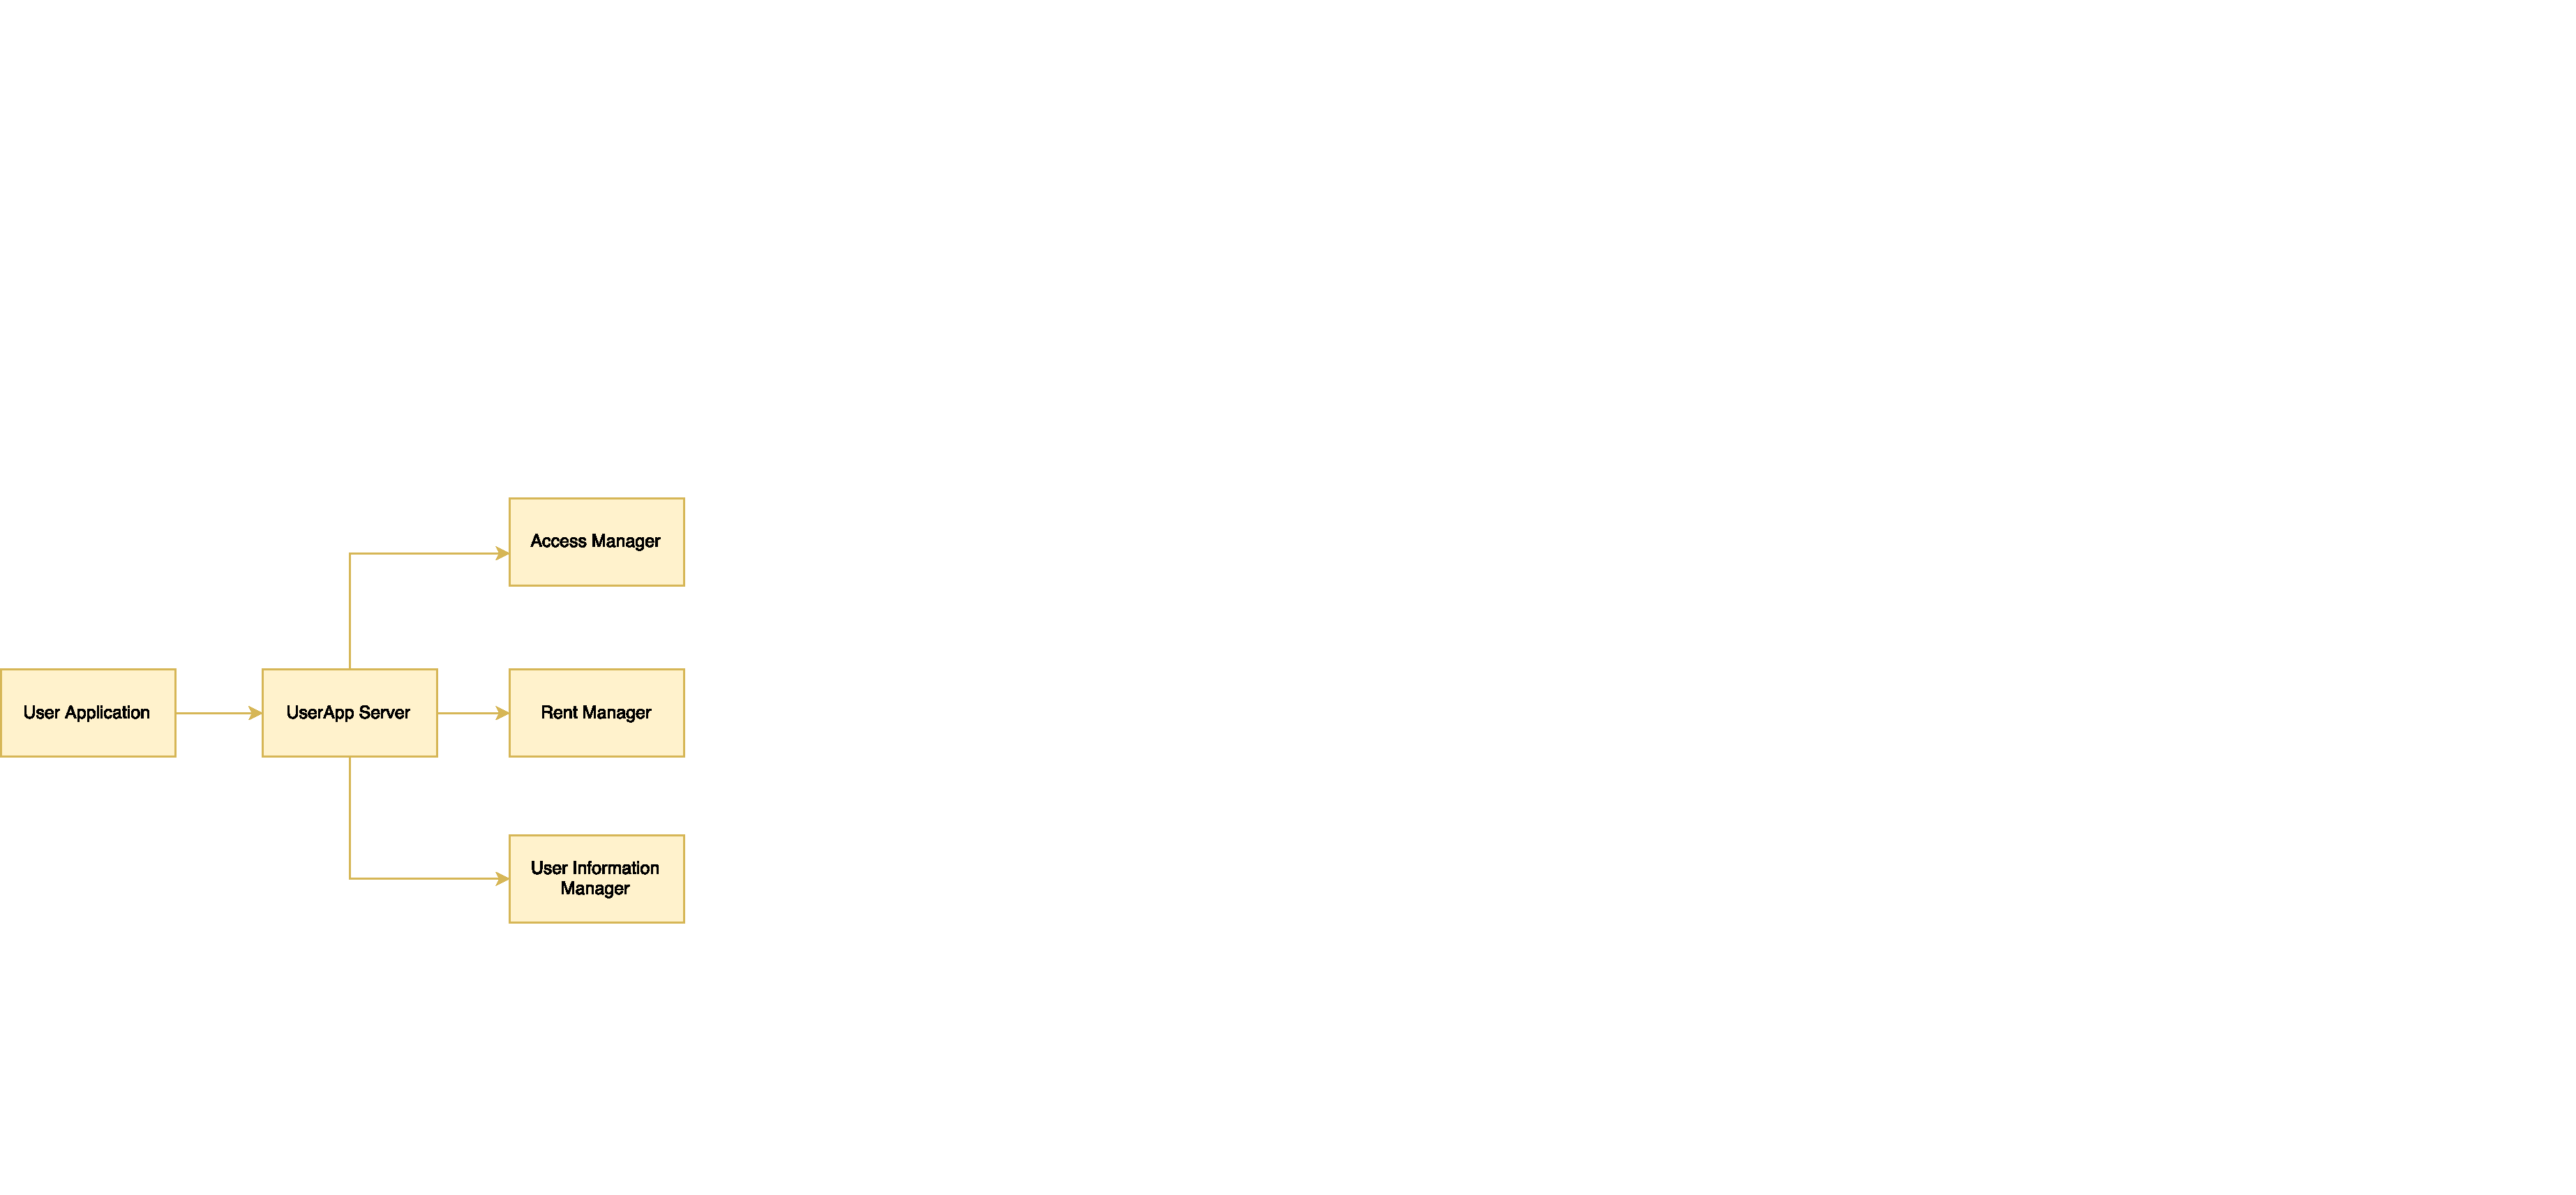
\includegraphics[width=0.8\linewidth]{img/Integration4}
			\caption{
				\label{fig:userAppServer} 
				\emph{User Application and Server integration}
			}
		\end{figure}

\clearpage 

\subsubsection{Subsystem Integration Sequence}

Unisco i sottosistemi del Maintenance (figura \ref{fig:maintenanceManager}), dello User (figura \ref{fig:userAppServer})  e del Customer Care (figura \ref{fig:ccAppServer}) nel sistema finale e testo tutto insieme. \todo{inglese}

	\begin{figure}[h]
			\centering
			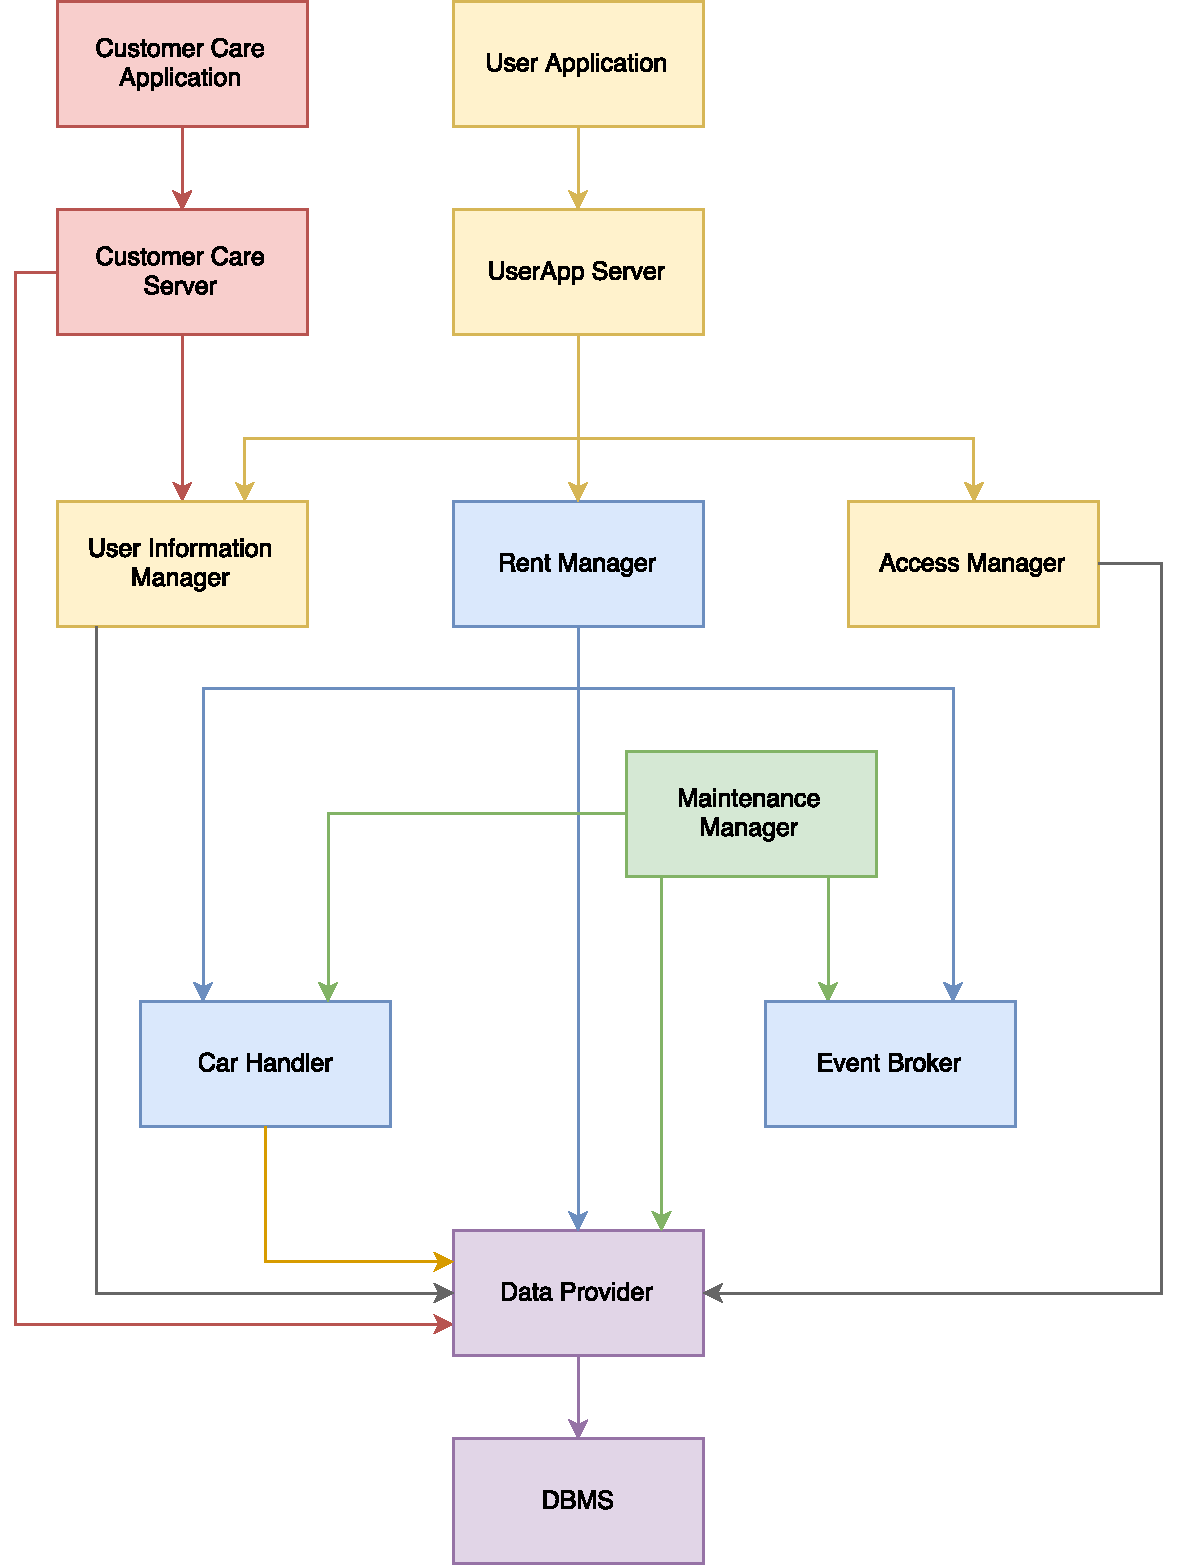
\includegraphics[width=0.8\linewidth]{img/subsystemIntegration}
			\caption{
				\label{fig:subsystemIntegration} 
				\emph{Subsystems Integration}
			}
		\end{figure}
